\chapter{Solución}

Teniendo clara una necesidad y/o problema a suplir/solucionar, se analizaron varias tecnologías y patrones de desarrollo que permitirían llevar a cabo el desarrollo de la aplicación y consecuentemente su puesta en marcha.

Las herramientas seleccionadas fueron, \textbf{Ruby on Rails}\footnote{http://rubyonrails.org/} para desarrollar la aplicación web, pensando en un metodología ágil de desarrollo, y que a su vez permitiera que los contenidos fueran fáciles de integrar, por otro lado, se elegió \textbf{Unity3D}\footnote{http://unity3d.com/} por su capacidad de generar contenidos 3D que se apoyan directamente de las tarjetas aceleradoras de video para visualizar dichas escenas, además cuenta con una API que facilita exportar contenidos para que sean visibles en un navegador.

\section{¿Por qué Ruby on Rails?}

Para responder a esta pregunta, es necesario primero definir a \textbf{Ruby on Rails}, llamado tambien \emph{Rails} ó RoR, es un \emph{framework} que hace que sea más fácil desarrollar, implementar, y mantener aplicaciones web. Durante los meses que siguieron a su primera liberación, \emph{Rails} paso de ser un juguete desconocido a un fenomeno mundial. Ha ganado premios, y más importante aún, se ha convertido en el framework de preferencia para la implementación de cierto conjunto de las llamadas aplicaciones Web 2.0\cite{ror:awdwr}.\\

Se eligió \emph{Rails} para desarrollar la aplicación web en la que se comunican datos y contenidos 3D, por qué se buscaba utilizar una herramienta en la que la convención estuviera por encima de la configuración\footnote{Léase \textbf{CoC} en el glosario}, que contará con una arquitectura pre definida, en éste caso MVC (Modelo Vista Controlador) Figura\ref{fig:mvc} que \emph{Rails} aprovecha apropiadamente, cuándo se desarrolla en \emph{Rails}, hay un lugar para cada pieza de código\footnote{Léase \textbf{DRY} en el glosario}, y todos los componentes de la aplicación interactúan según el estándar.\\

\begin{figure}[h]
	\centering
		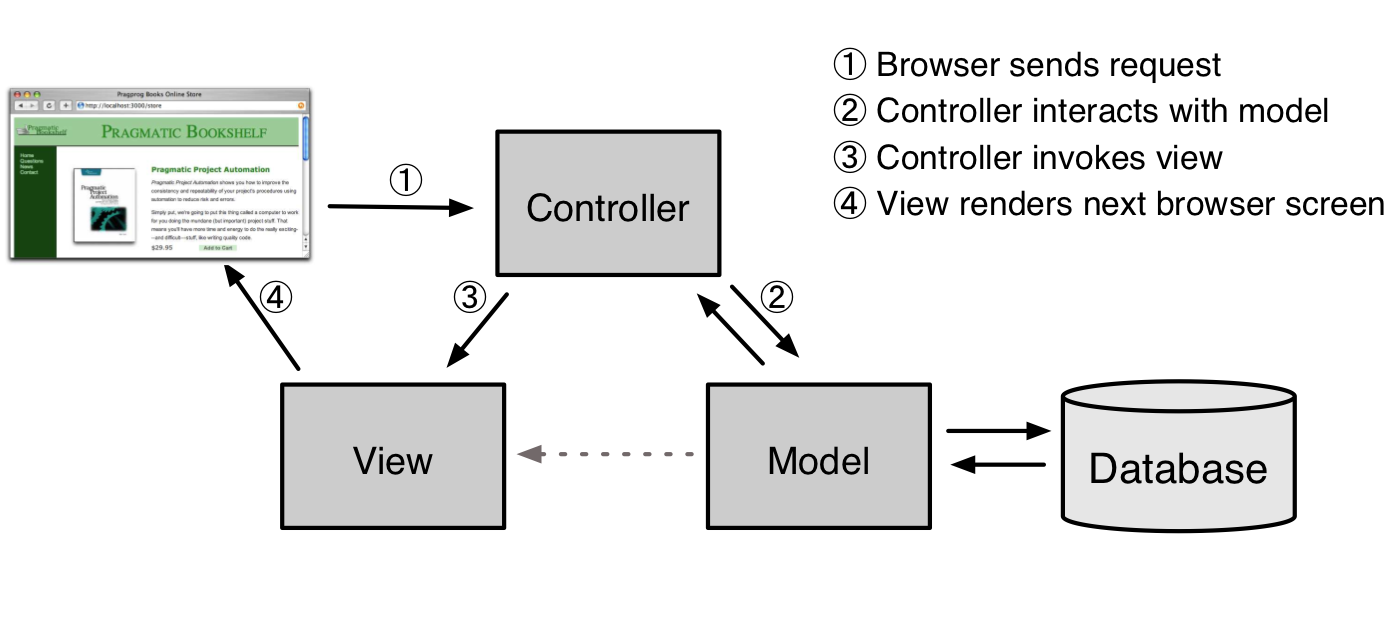
\includegraphics[scale=0.25]{mvc.PNG}
		\caption{Modelo Vista Controlador}
	\label{fig:mvc}
\end{figure}

Los programadores profesionales, suelen escribir tests para simular el comportamiento de la aplicación que se esta desarrollando, para el presente proyecto, se buscaba que el framework tuvieran un soporte para hacer tests, una vez más Rails se ajusta a esas necesidades, pues cuenta con soporte para algunos frameworks para realizar tests, se encuentran; RSpec (utilizada en este proyecto, bajo la filosofía de TDD \footnote{Léase \textbf{TDD} en el glosario}) en donde se escriben los tests, antes de la implementación, Test Unit, Shoulda y Cucumber (BDD\footnote{Léase \textbf{BDD} en el glosario})\\

Se buscaba que la herramienta fuera escrita en un lenguaje de programación orientado a objetos e interpretado, por la necesidad de crear \emph{scripts} que corrieran independiente de la aplicación, como tareas programadas para correr cada cierto tiempo. Las aplicaciones en \emph{Rails} son escritas en el lenguaje de programación \emph{Ruby}, que cumple con lo que se buscaba, y aparte introduce características favorables como metaprogramación, haciendo que el código sea más fácil de entender, leer y/o escribir, programas más cortos en términos de \textbf{LOC}\footnote{Líneas de código, en inglés \emph{Lines of Code}}, para evidenciar esto, a continuación se muestra una porción de código de la aplicación, en la que se define una clase de un Modelo que expresa mucha información en pocas líneas de código y es fácil de entender. \newpage

\begin{verbatim}
class Record < ActiveRecord::Base  

  belongs_to :stock_action

  validates_presence_of :amount
  validates_presence_of :price
  validates_presence_of :variation

  validates_numericality_of :price, :amount, :greater_than => 0
  validates_numericality_of :variation

end
\end{verbatim}

Finalmente, no se pretendía manipular la base de datos directamente, es decir, con código nativo del motor de bases de datos, sino sacar provecho de técnicas como ORM \footnote{Léase \textbf{ORM} en el glosario}, en las que las tablas de las bases de datos son mapeadas a clases, los registros de las tablas son mapeados como objetos, y consecuentemente los campos, se mapean como atributos de los objetos, mientras que existen metodos de clases que se encargan de realizar operaciones a nivel de tablas, dejando como opcional la utilización de código \textbf{SQL} dentro de la aplicación, una vez más \emph{Rails} suple esta necesidad con \textbf{ActiveRecord} ó \textbf{Datamapper}.

\section{¿Por qué Unity3D?}

Actualmente existen posibilidades para el desarrollo de interfaces gráficas de usuario tridimensionales en los navegadores de internet, \textbf{PaperVision3D}\footnote{\textbf{Papervision} es un motor de gráficos para Flash. Aunque todavía está en versión beta, ya se han lanzado algunas aplicaciones que lo utilizan y los resultados son muy prometedores.} (entre otros) es un motor de renderizado 3D en tiempo real, escrito en \textbf{ActionScript 3}\footnote{\textbf{ActionScript} es un lenguaje de programación orientado a objetos (OOP), utilizado en especial en aplicaciones web animadas realizadas en el entorno \textbf{Adobe Flash}}, de código abierto entre otros, que posee las funcionalidades básicas de la computación gráfica tridimensional, creando una ilusión 3D en el motor de renderizado que posee el \emph{Flash Player}. \\

Desafortunadamente el motor de renderizado para \emph{Flash} esta diseñado específicamente para gráficos en 2D. Este es un punto crítico por el cual \emph{Flash} no es técnicamente la mejor opción. La cantidad de fotogramas de contenido 3D renderizados por segundo (FPS)\footnote{Las imágenes por segundo (en inglés más conocido como \emph{frames per second, fps}) es la medida de la frecuencia a la cual un reproductor de imágenes genera distintos fotogramas (\emph{frames}). En informática estos fotogramas están constituídos por un número determinado de pixeles que se distribuyen a lo largo de una red de texturas para determinar un fotograma por segundo.\\
La frecuencia es proporcional al número de pixeles que se deben generar, incidiendo en el rendimiento de la máquina.} suele ser media o baja, en casos reales. La comunidad de desarrolladores del \emph{Flash Player} está desarrollando varios proyectos para poder renderizar 3D en el mismo, existen proyectos privados y de código abierto, entre los que se encuentran: \\
\begin{itemize}
\item[$\bullet$] \emph{Alternativa3D} 
\item[$\bullet$] \emph{Away 3D} 
\item[$\bullet$] \emph{Five3D} 
\item[$\bullet$] \emph{ND3D} 
\item[$\bullet$] \emph{Papervision3D} 
\item[$\bullet$] \emph{Sandy3D} 
\item[$\bullet$] \emph{Wire Engine 3D}
\end{itemize} 
Los cuales usualmente utilizan algoritmos de rasterizado para el proceso de generar una imagen 2D a partir de una escena 3D, consumiendo así en dicho proceso, mucha capacidad computacional.\\

La técnica más utilizada hoy en día para la producción de gráficos 3D en tiempo real es la rasterización. La rasterización es básicamente un proceso de transformación de datos de vectores que se convierten en un conjunto de pixeles (imágenes).\\

En pocas palabras, muchos de los motores de renderizado 3D escritos para trabajar con el \emph{plugin} de \emph{Flash}  utilizan bastante lógica para producir una ilusión 3D sobre 2D debido a que es una de las técnicas mas rápidas, pero, como se mencionó anteriormente, estos motores por mas optimizados que estén, siempre van a depender del renderizado 2D para el cual fue diseñado \emph{Flash} en un principio.\\

\textbf{Unity3D} por su parte también es un \emph{plugin} para navegadores, especializado en la creación de contenido 3D en tiempo real. Técnicamente es la mejor opción para desarrollo 3D, pues dicho \emph{plugin} aprovecha las capacidades de procesamiento de hardware de la tarjeta de video para desplegar contenidos en 3D, permitiendo así optimizar ciclos de procesamiento en el mejoramiento de los FPS de la escena en vez de ejecutar cálculos de conversión de imágenes 3D a 2D, repercutiendo enormemente en la experiencia del usuario.\\

\emph{Unity3D} por su parte es un motor escrito en C/C++ que trabaja con \emph{Mono}\footnote{\textbf{Mono} es el nombre de un proyecto de código abierto iniciado por Ximian y actualmente impulsado por Novell (tras la adquisición de Ximian) para crear un grupo de herramientas libres, basadas en GNU/Linux y compatibles con .NET según lo especificado por el ECMA.} y \emph{PhysX}\footnote{\textbf{PhysX} es un chip y un kit de desarrollo diseñados para llevar a cabo cálculos físicos muy complejos. Conocido anteriormente como la SDK de NovodeX, fue originalmente diseñada por AGEIA y tras la adquisición de AGEIA, es actualmente desarrollado por Nvidia e integrado en sus chip gráficos más recientes.} para crear código multiplataforma, haciendo así practicamente transparente generar ejecutables tanto para MacOSX, Windows, widgets y exportar para Web.\\

Gracias a Mono, es fácil generar ejecutables multiplataforma debido a la arquitectura con la que dicho \emph{framework} trabaja.Figura\ref{fig:mono}\\

\begin{figure}[h]
	\centering
		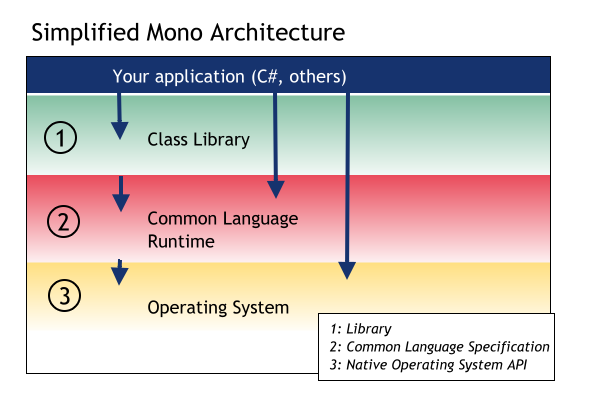
\includegraphics[scale=0.7]{Mono.PNG}
		\caption{Arquitectura general del \emph{framework} Mono}
	\label{fig:mono}
\end{figure}


Por otro lado, \emph{Unity3D} también se aprovecha de la capacidad del motor de física \emph{PhysX} para llevar a cabo cálculos complejos para así alivianar la carga de procesamiento que conlleva un juego/aplicación 3D.\\

Cuando el Motor exporta contenido a Web, dicho contenido se puede comunicar facilmente con \emph{Javascript}, permitiendo así entablar un puente de comunicaciones con \emph{Rails} a través de \emph{Javascript}, factor clave para la visualización de los datos que tiene la aplicación.\\

